\documentclass[10pt, conference, compsocconf]{IEEEtran}
\ifCLASSINFOpdf
\else
\fi
\usepackage[pdftex]{graphicx}  
\graphicspath{ {images/} } 
\usepackage[hidelinks]{hyperref}
\usepackage{array}
\usepackage{algorithm,algcompatible,amsmath}
\DeclareMathOperator*{\argmax}{\arg\!\max}% https://tex.stackexchange.com/q/83169/5764
\algnewcommand\INPUT{\item[\textbf{Input:}]}%
\algnewcommand\OUTPUT{\item[\textbf{Output:}]}%
\hyphenation{op-tical net-works semi-conduc-tor}

\begin{document}
\title{Long Short-Term Memory to predict parking space in Denmark }
\author{\IEEEauthorblockN{Alkharif Sarah}
\IEEEauthorblockA{M2016426\\
sara.alabdulaziz@gmail.com}}
\maketitle
\begin{abstract}
The smart parking is in smart city aims to facilitate users with accurate information regarding available parking spots. The prediction of available parking spots in next time steps for parking using deep learning can facility improved accuracy of occupancy status, efficient traffic management and better utilization of parking lots. Using Long Short-term Memory (LSTM) algorithm to predict time series data sets, and we applied our data set to other statistical models for time series prediction compare their performance; we measure the performance with Root-Mean-Square Error RMSE,
the result shows that our model works more efficiently.
\end{abstract}
\IEEEpeerreviewmaketitle
\section{Introduction}
The deep learning is a promising field through which systems can learn to classify or predict solution for particular give problem based on input data. There are real time parking prediction systems available but unable to provide prediction for multi-step or forecasting in cases if user is far away from parking spot or has encountered a certain situation. The deep learning can resolve this issue by learning from data for future forecasting. Thus, it brings positivize hopes towards predicting occupancy rate and deploying in smart parking setting.

\section{Model}

\subsection{Statistacl Models}
In this work, we use some classical time-series analysis algorithms to predict future parking lots. First, autoregressive model AR, is the number of auto-regressive terms that indicates dependencies on past values,AR model of order \(p\) where the  \(p\) is number of lagged, can be written as''
\begin{equation}
\hat{y_t} = w_0 +\beta_1 y_{t-1}+ \beta_2 y_{t-2}+.....\beta_n y_{t-n}+\epsilon_t
\label{Eq-AR}
\end{equation}
where  \(w-0\) is a constant and \(\beta\) is white noise, with error tearm.


Moving Avrage MA is a statistical model that computes white noise based on previous white noise, which has the general form in Equation below:

\begin{equation}
\hat{y_t} = w_0 +\epsilon_t + \delta_1 \epsilon_{t-1}+  \delta_2 \epsilon_{t-2}+...+ \delta_n \epsilon_{t-n}
\label{Eq-MA}
\end{equation}
where \(w-0\) is a constant mean, \(\delta\) is a coefficient, t is time, where the curent obesrvation depends on past observation known as number of lags, and \(\epsilon\) is an error term.

\subsection{Deep learning Model}
The benefit of LSTM is cell unit, it is tries to remember the most crucial point in data. LSTM developed to fix the exploding and vanishing gradient when training RNN; by using a memory unit known as a cell unit or cell memory \(c_t\)  for a network. Cell unit allowed to remember the output, which helps the model to learn from all output of the sequence data.
\ref{fig:LSTM} shows the most essential three gates of LSTM model: \(update\) gate,\(forget\) gate and \( output \) gate. LSTM can be described by Equations (1-6). First \(\hat c_t\) which is a candidate that can append to the memory cell, that can be computed by using
 Equation \ref{c}. \(update\) gate. Equation \ref{update} helps the model to decide when it can update the cell state by using a sigmoid function; if the output is close to one, it is updated, if it it close to zero, it is ignored. It is same as \(forget\) gate that allows the model to chose when to forget the information in cell state, as shown in Equation \ref{foreget}. The \(output \) gate,  which is computed in Equation \ref{output}, \(c_t\) where we get the new cell state to transfer it to the next layer by multiply \(update\) gate with candidate $\hat c_t$ and added to \(foreget\) gate that multiply with previous  cell state \ref{cell}. Finally we have to prepare \(a_t\) to send it to the next layer using Equation \ref{a}, to keep tracking the parameters.
\begin{figure}[h]
 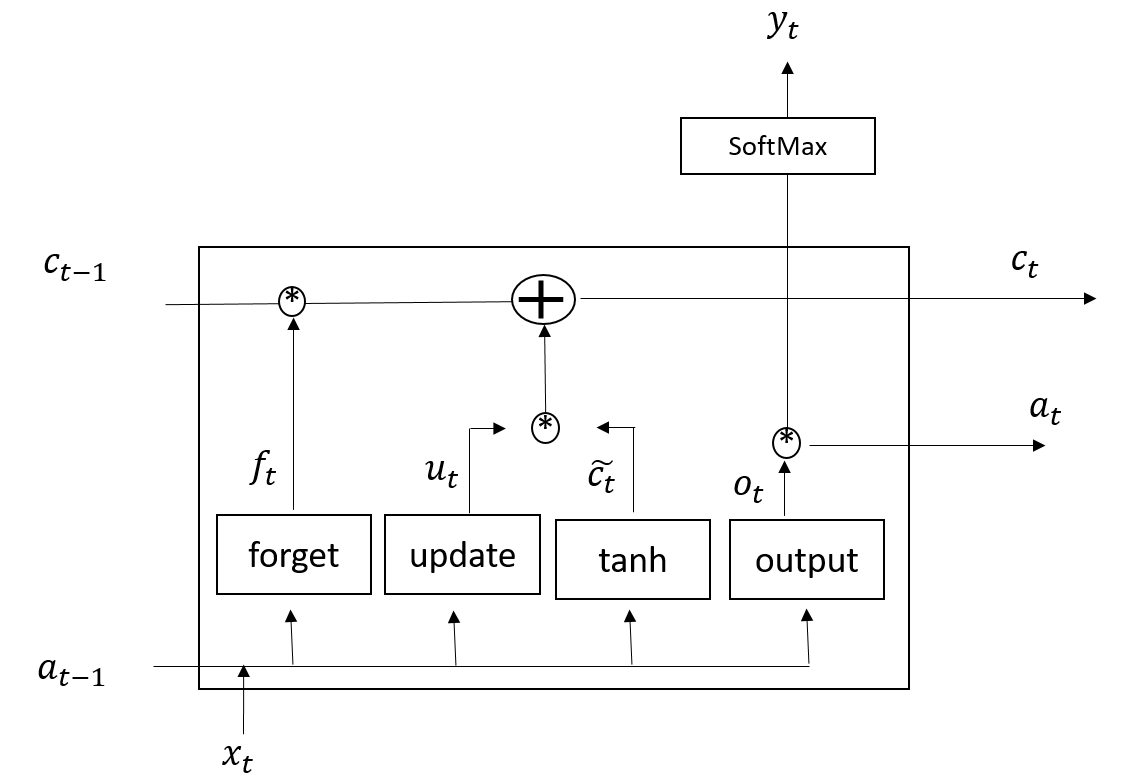
\includegraphics[width=6.1cm, height=5.5cm]{lstm}
 \caption{\footnotesize The diagram of a LSTM building block}
 \label{fig:LSTM}
\end{figure}
\begin{equation} \label{c} 
 \hat c_t= \tanh{(W_c[a_{t-1},x_t]+b_c)}
\end{equation}
\begin{equation} \label{update} 
 u_t= \sigma{(W_u[a_{t-1},x_t]+b_u)}
\end{equation}
\begin{equation} \label{foreget} 
 f_t= \sigma{(W_f[a_{t-1},x_t]+b_f)}
\end{equation}
\begin{equation} \label{output} 
 o_t= \sigma{(W_o[a_{t-1},x_t]+b_o)}
 \end{equation}
\begin{equation} \label{cell} 
 c_t= u_t* \hat c_t +f_t* c_{t-1}
 \end{equation}
 \begin{equation} \label{a} 
 a_t= o_t *\tanh( c_t)
 \end{equation}
\section{Evaluation}
We collected datasets for our project from citypulse website. A data-stream with parking data provided from the city of Aarhus. There are a total of 8 parking lots providing information over a period of 6 months (55.264 data points in total). From May 22, 2014 to November 4,2014. Then we get an hourly occupied it that can make an hourly forecast, and  we get the  mormlaize value; we set our target $\hat y$ as next hour occupied. We used 80\% and 20\% of the dataset for training and testing, respectively, then run LSTM model individually for every parking to get output $\hat y $.  then measure the performance by using root-mean-square error (RMSE) with actual value \(Y\) to get the average error for every parking. We applied the data set to other statistical models as AR and MA time series prediction model to compare their performance. 
We implemented the work using python 3.6.2 and Anaconda open source distribution 4.4.7. To run the model, we used Keras, which is a high-level neural networks API, running on top of TensorFlow. We set our model parameters with four hidden units and one layer which best chose. The results given in Table \ref{table:1} show the  performance of the 3 models.
\begin{figure}[h]
 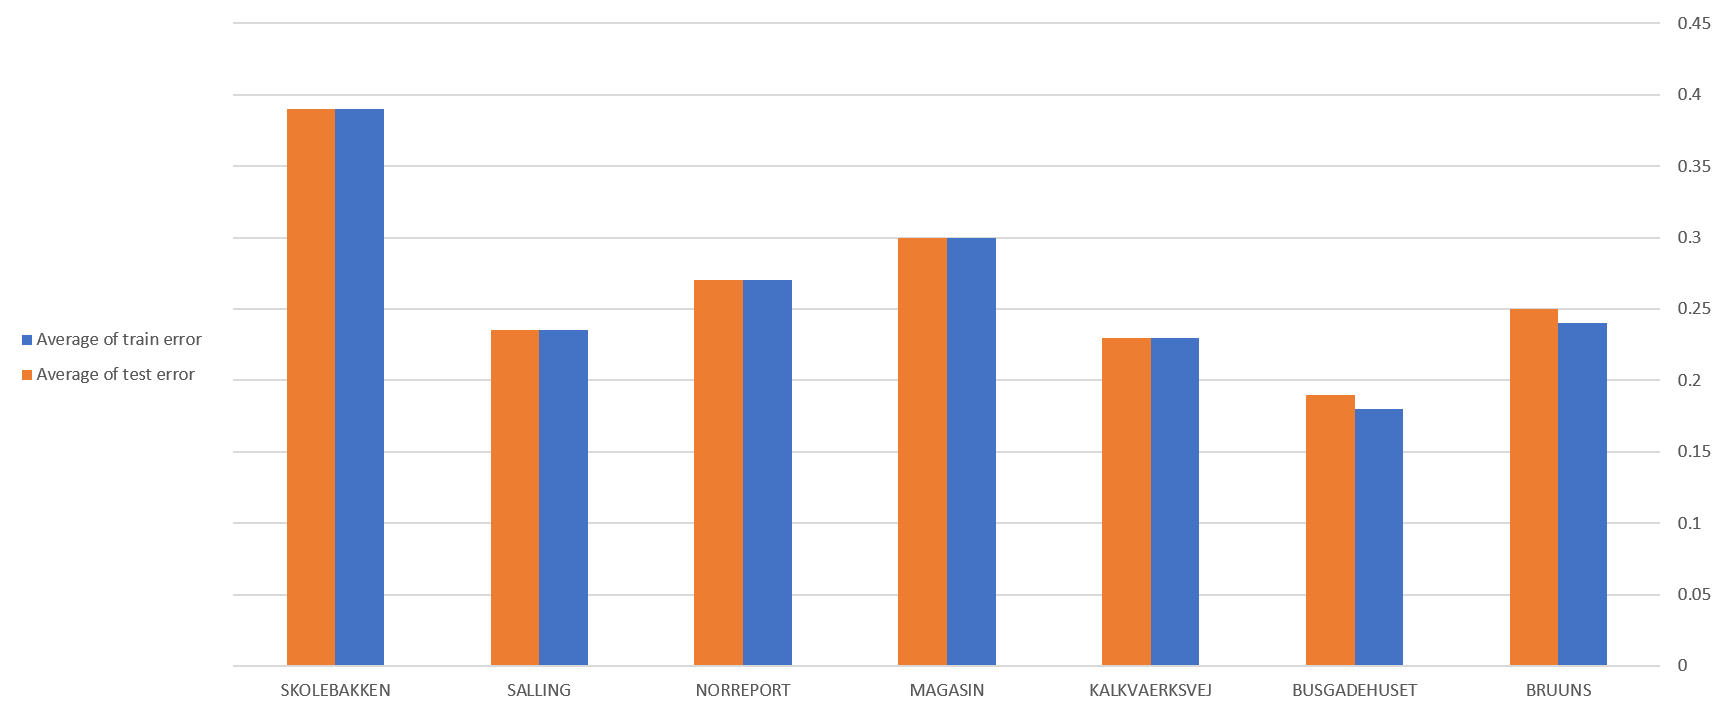
\includegraphics[width=7.1cm, height=4.5cm]{result}
 \caption{\footnotesize The LSTM model result}
 \label{fig:result}
\end{figure}
\begin{table}[h!]
\begin{tabular}{ | m{3cm} | m{1cm}| m{1cm} | m{1cm} | } 
\hline
Parking name & MA & AR& LSTM\\ 
\hline
BRUUNS& 0.96 & 0.97 &0.24\\ 
\hline
BUSGADEHUSET & 0.92 & 0.92&0.19 \\ 
\hline
KALKVAERKSVEJ & 0.89 & 0.89 &0.23\\ 
\hline
MAGASIN & 1.03 & 1.02& 0.30\\ 
\hline
NORREPORT & 0.70 &0.70 &0.27\\ 
\hline
SALLING & 1.02 & 0. 1.03&0.25\\ 
\hline
SCANDCENTER & 1.05 & 0.1.05& 0.22\\ 
\hline
SKOLEBAKKEN & 1.39 & 1.05& 0.39\\ 
\hline
\end{tabular}

\caption{\footnotesize the train set RMSE for 8 parking.}
\label{table:1}
\end{table}
\section{Conclusion}
To predict parking space in Denmark we apply Deep Learning algorithem LSTM model to the data for all 8 parking, and we applied our data set to other statistical models for time series prediction compare their performance, using root-mean-square error to evaluate the performance, we found that LSTM model work more efficiently.
\end{document}


